\documentclass[11pt,a4paper]{article}

% Packages
\usepackage[utf8]{inputenc}
\usepackage[T1]{fontenc}
\usepackage[french]{babel}
\usepackage{amsmath,amssymb,amsfonts}
\usepackage{graphicx}
\usepackage{geometry}
\usepackage{fancyhdr}
\usepackage{hyperref}
\usepackage{xcolor}
\usepackage{listings}
\usepackage{booktabs}
\usepackage{caption}
\usepackage{float}
\usepackage{algorithm}
\usepackage{algpseudocode}

% Page geometry
\geometry{top=2.5cm, bottom=2.5cm, left=2.5cm, right=2.5cm}

% Colors
\definecolor{darkblue}{RGB}{31,56,100}
\definecolor{medblue}{RGB}{46,117,182}
\definecolor{codebg}{RGB}{245,245,245}
\definecolor{codegreen}{RGB}{40,120,40}

% Header/footer
\pagestyle{fancy}
\fancyhf{}
\fancyhead[L]{\small\textcolor{gray}{MOR 2025 -- (MS)$^2$SC}}
\fancyhead[R]{\small\textcolor{gray}{\textit{Séance 2 : PGD pour l'équation de la chaleur}}}
\fancyfoot[C]{\thepage}
\renewcommand{\headrulewidth}{0.4pt}

% Code listing style
\lstset{
  language=Matlab,
  basicstyle=\small\ttfamily,
  backgroundcolor=\color{codebg},
  frame=single,
  rulecolor=\color{gray!30},
  keywordstyle=\color{medblue}\bfseries,
  commentstyle=\color{codegreen}\itshape,
  stringstyle=\color{red!60!black},
  breaklines=true,
  numbers=none,
  xleftmargin=4pt,
  xrightmargin=4pt,
  aboveskip=8pt,
  belowskip=8pt,
}

% Section formatting
\usepackage{titlesec}
\titleformat{\section}{\Large\bfseries\color{darkblue}}{\thesection}{1em}{}
\titleformat{\subsection}{\large\bfseries\color{medblue}}{\thesubsection}{1em}{}

\begin{document}

% ============ TITLE PAGE ============
\begin{titlepage}
\centering
\vspace*{2cm}
{\Huge\bfseries\textcolor{darkblue}{Séances pratiques MOR}\par}
\vspace{0.5cm}
{\LARGE\textcolor{darkblue}{Rapport -- Séance 2}\par}
\vspace{1.5cm}
{\Large Résolution de l'équation de la chaleur instationnaire\par}
{\large par Décomposition Propre Généralisée (a priori)\par}
\vspace{2cm}
{\large ENS Paris-Saclay -- Master (MS)$^2$SC\par}
\vspace{0.5cm}
{\large Encadrant : Eren Alagoz\par}
\vspace{2cm}
{\large \textbf{Auteurs :} Achraf Benmalk, Binôme\par}
\vspace{1cm}
{\large \today\par}
\end{titlepage}

% ============ TABLE OF CONTENTS ============
\tableofcontents
\newpage

% ============================================================
\section{Énoncé du problème}
% ============================================================

Nous considérons l'équation de la chaleur 1D instationnaire sur une barre $\Omega = [0, L]$
sur l'intervalle de temps $I = [0, T]$ :
\begin{equation}
    \rho c \frac{\partial u}{\partial t} - k \frac{\partial^2 u}{\partial x^2} = f(x,t)
    \quad \text{dans } \Omega \times I
    \label{eq:heat}
\end{equation}
avec des conditions aux limites de Dirichlet oscillantes
$u(0,t) = \sin(2\pi t / T)$ et $u(L,t) = -\sin(4\pi t / T)$,
et la condition initiale $u(x,0) = 0$.

Les paramètres physiques sont $\rho = c = k = 1$, $L = 1$, $T = 2$,
avec $n_X = 300$ nœuds spatiaux et $n_T = 100$ pas de temps.
Le chargement volumique $f$ est choisi aléatoirement.

L'objectif est de résoudre cette équation par la méthode PGD et de comparer le résultat
avec une solution de référence par éléments finis classiques.

% ============================================================
\section{Solution de référence : Éléments Finis + Euler implicite}
% ============================================================

\subsection{Discrétisation spatiale}

Nous approchons $u(x,t) \approx \sum_j U_j(t)\,\varphi_j(x)$ au moyen de fonctions
de chapeau P1 $\varphi_j$. La formulation faible de Galerkin standard conduit au système
semi-discret :
\begin{equation}
    M\dot{U}(t) + KU(t) = F(t)
    \label{eq:semidiscrete}
\end{equation}
où $M_{ij} = \int_\Omega \rho c\,\varphi_i\varphi_j\,dx$ est la matrice de masse consistante,
$K_{ij} = \int_\Omega k\,\varphi_i'\varphi_j'\,dx$ la matrice de rigidité,
et $F_i = \int_\Omega f\,\varphi_i\,dx$ le vecteur de chargement.

\subsection{Opérateurs d'intégration}

Pour calculer les normes $L^2$ et les produits scalaires en espace et en temps,
nous assemblons des matrices d'intégration consistantes en bouclant sur les éléments.
La matrice de masse élémentaire locale vaut
$\frac{h}{6}\begin{pmatrix}2&1\\1&2\end{pmatrix}$,
assemblée globalement :
\begin{lstlisting}
Ix = zeros(n_X); It = zeros(n_T);
Ie_x = dx * [1/3, 1/6; 1/6, 1/3];
Ie_t = dt * [1/3, 1/6; 1/6, 1/3];
for i = 1:(n_X - 1)
    Ix(i:i+1, i:i+1) = Ix(i:i+1, i:i+1) + Ie_x;
end
for i = 1:(n_T - 1)
    It(i:i+1, i:i+1) = It(i:i+1, i:i+1) + Ie_t;
end
\end{lstlisting}
Chaque élément contribue sa matrice locale $2\times2$ à la matrice globale aux degrés de liberté
correspondants. L'assemblage par superposition produit naturellement la structure tridiagonale.

\subsection{Schéma d'Euler implicite}

Le schéma d'Euler implicite (rétrograde) approche
$\dot{U}(t_i) \approx (U_i - U_{i-1})/\Delta t$ :
\begin{equation}
    \underbrace{\left(\frac{M}{\Delta t} + K\right)}_{H} U_i
    = F(t_i) + \frac{M}{\Delta t}U_{i-1}
    \label{eq:euler}
\end{equation}
Ce schéma est inconditionnellement stable, ce qui nous permet de choisir $\Delta t$
librement sans contrainte CFL, à la différence d'un schéma explicite.

\subsection{Conditions aux limites par substitution}

Les conditions aux limites de Dirichlet non nulles sont imposées par la méthode de
substitution. Les degrés de liberté sont séparés en DDL bloqués
$\text{ddld} = \{1, n_X\}$ et DDL libres $\text{ddlu}$.
À chaque pas de temps, le système est résolu uniquement sur les DDL libres :
\begin{lstlisting}
for i = 2:n_T
    G = F(:,i) + (M/dt)*Uex(:,i-1);
    Uex(ddlu,i) = H(ddlu,ddlu) \ (G(ddlu) - H(ddlu,ddld)*Uex(ddld,i));
end
\end{lstlisting}
Le terme $H(\text{ddlu},\text{ddld}) \cdot U_{\text{ex}}(\text{ddld},i)$ transfère
l'influence des valeurs connues aux frontières vers le second membre.

% ============================================================
\section{Changement de variable}
% ============================================================

\subsection{Motivation}

La PGD cherche $W(x,t) = \sum_i \Lambda_i(x)\cdot\lambda_i(t)$ où chaque mode spatial
$\Lambda_i$ doit s'annuler aux frontières pour appartenir à l'espace admissible.
Puisque la solution réelle $U$ possède des conditions aux limites non nulles,
nous ne pouvons pas appliquer directement la PGD à $U$.

\subsection{Décomposition de la solution}

Nous décomposons $U = U_{CL} + W$ où $U_{CL}$ est un champ
\og dynamiquement admissible \fg{} qui satisfait les conditions aux limites et initiales,
et $W$ est le reste avec des conditions aux limites homogènes
($W(0,t) = W(L,t) = 0$).

Le choix le plus simple est une interpolation linéaire :
\begin{equation}
    U_{CL}(x,t) = \left(1 - \frac{x}{L}\right)\sin\!\left(\frac{2\pi t}{T}\right)
    + \frac{x}{L}\left(-\sin\!\left(\frac{4\pi t}{T}\right)\right)
    \label{eq:ucl}
\end{equation}
En MATLAB, cela se calcule par un produit extérieur :
\begin{lstlisting}
u_cl = (1 - lx'/L) * Ud0 + (lx'/L) * UdL;
\end{lstlisting}

\subsection{Équation pour $W$}

En substituant $U = U_{CL} + W$ dans (\ref{eq:semidiscrete}) :
\begin{equation}
    M\dot{W} + KW = \underbrace{F - M\dot{U}_{CL} - KU_{CL}}_{Q_0}
    \label{eq:weq}
\end{equation}
La dérivée temporelle $\dot{U}_{CL}$ est calculée au moyen d'un opérateur de
différences finies agissant à droite :
\begin{equation}
    \mathbb{D}_t = \frac{1}{\Delta t}
    \begin{pmatrix} 1 & -1 & & \\ & 1 & -1 & \\ & & \ddots & \ddots \end{pmatrix}
\end{equation}
de sorte que \texttt{u\_cl\_dot = u\_cl * Dt} calcule la dérivée temporelle pour
chaque nœud spatial simultanément. Le second membre modifié est alors :
\begin{lstlisting}
Dt = (1/dt) * (eye(n_T) + diag(-ones(n_T-1,1), 1));
u_cl_dot = u_cl * Dt;
G0 = F - M*u_cl_dot - K*u_cl;
\end{lstlisting}

\subsection{Validation}

Nous résolvons l'équation modifiée (\ref{eq:weq}) pour $W$ avec le même schéma
d'Euler implicite, puis nous récupérons $U_1 = W + U_{CL}$.
La différence $\|U_1 - U_{\text{ex}}\|$ est de l'ordre de $10^{-12}$,
ce qui confirme que les deux approches résolvent bien le même problème.

% ============================================================
\section{Résolution par PGD}
% ============================================================

\subsection{Principe de la représentation séparée}

Au lieu d'avancer pas à pas en temps, la PGD cherche $W$ sous la forme d'une somme
de modes espace-temps séparés :
\begin{equation}
    W(x,t) = \sum_{i=1}^{m} \Lambda_i(x)\cdot\lambda_i(t)
    \label{eq:pgd_sep}
\end{equation}
Chaque mode $(\Lambda_i, \lambda_i)$ est calculé de manière gloutonne, un par un,
par une alternance de point fixe entre un problème EF spatial et une EDO temporelle.
L'intérêt est d'éviter de construire et de résoudre le système espace-temps global
de taille $N_x \times N_T$, ce qui serait prohibitif.

\subsection{Formulation faible espace-temps}

L'approximation PGD est insérée dans la formulation faible espace-temps de
(\ref{eq:weq}). En testant par $(\Lambda\lambda^* + \Lambda^*\lambda)$, où
$\lambda^*$ et $\Lambda^*$ sont des variations arbitraires :
\begin{equation}
    \int_0^T (\Lambda\lambda^* + \Lambda^*\lambda)^\top
    \left[M\Lambda\dot{\lambda} + K\Lambda\lambda - Q(t)\right]dt = 0
    \label{eq:pgd_weak}
\end{equation}
où $Q = Q_0 - M\dot{W}_{\text{prec}} - KW_{\text{prec}}$ est le résidu courant
(contribution des modes déjà calculés).

\subsection{Algorithme de point fixe}

Le problème étant non linéaire dans la paire $(\Lambda, \lambda)$,
nous alternons entre deux sous-problèmes linéaires :

\subsubsection{Problème spatial ($\lambda$ fixé)}

En posant $\lambda^* = 0$ dans (\ref{eq:pgd_weak}) et en supprimant
$\Lambda^*$ arbitraire :
\begin{equation}
    \underbrace{\left[\left(\int_0^T \lambda\dot{\lambda}\,dt\right)M
    + \left(\int_0^T \lambda^2\,dt\right)K\right]}_{\mathbb{J}} \Lambda
    = \underbrace{\int_0^T Q(t)\lambda\,dt}_{q}
    \label{eq:fe_problem}
\end{equation}
Les intégrales en temps sont des scalaires calculés à partir du $\lambda$ connu,
donc $\mathbb{J}$ est une combinaison linéaire de $M$ et $K$ ---
un système EF standard de taille $N_x \times N_x$ résolu uniquement sur les DDL libres.
Après résolution, $\Lambda$ est normalisé :
$\Lambda \leftarrow \Lambda / \sqrt{\Lambda^\top I_x \Lambda}$.

En MATLAB, avec \texttt{lambdatmp} comme vecteur ligne $1 \times n_T$ :
\begin{lstlisting}
J = [lambdatmp*Dt*It*lambdatmp']*M + [lambdatmp*It*lambdatmp']*K;
q = lambdatmp * It * Q';
LAMBDAtmp = zeros(n_X, 1);
LAMBDAtmp(ddlu) = J(ddlu,ddlu) \ q(ddlu)';
LAMBDAtmp = LAMBDAtmp / sqrt(LAMBDAtmp'*Ix*LAMBDAtmp);
\end{lstlisting}

\subsubsection{Problème temporel ($\Lambda$ fixé)}

En posant $\Lambda^* = 0$ et en supprimant $\lambda^*$ arbitraire :
\begin{equation}
    \underbrace{\Lambda^\top M\Lambda}_{\alpha}\,\dot{\lambda}
    + \underbrace{\Lambda^\top K\Lambda}_{\beta}\,\lambda
    = \underbrace{\Lambda^\top Q(t)}_{\gamma(t)}
    \label{eq:ode}
\end{equation}
Il s'agit d'une EDO scalaire résolue par Euler implicite à coût négligeable :
\begin{equation}
    \lambda_i = \frac{\gamma(t_i)\Delta t + \alpha\,\lambda_{i-1}}{\alpha + \beta\,\Delta t}
\end{equation}

\begin{lstlisting}
alpha = LAMBDAtmp'*M*LAMBDAtmp;
beta  = LAMBDAtmp'*K*LAMBDAtmp;
gamma = LAMBDAtmp'*Q;
lambdatmp = zeros(1, n_T);
for i = 2:n_T
    lambdatmp(i) = (gamma(i) + (alpha/dt)*lambdatmp(i-1)) / ((alpha/dt) + beta);
end
\end{lstlisting}

\subsubsection{Critère de stagnation}

L'alternance est stoppée lorsque $\lambda$ n'évolue plus significativement :
\begin{equation}
    s = \frac{\int_0^T (\lambda^{\text{nouv}} - \lambda^{\text{anc}})^2\,dt}
    {\int_0^T (\lambda^{\text{anc}})^2\,dt}
    = \frac{(\lambda^{\text{nouv}}-\lambda^{\text{anc}})\,I_t\,
    (\lambda^{\text{nouv}}-\lambda^{\text{anc}})^\top}
    {\lambda^{\text{anc}}\,I_t\,(\lambda^{\text{anc}})^\top} < 10^{-5}
\end{equation}

\subsection{Algorithme glouton}

L'algorithme PGD complet est résumé ci-dessous.

\begin{algorithm}[H]
\caption{PGD Glouton (sans mise à jour)}
\begin{algorithmic}[1]
\State Initialiser $W = 0$, $Q_0 = F - M\dot{U}_{CL} - KU_{CL}$
\For{$\text{mode} = 1, 2, \ldots, n_{\text{modes}}$}
    \State Mettre à jour le résidu : $Q = Q_0 - M\dot{W} - KW$
    \State Initialiser $\lambda$ (ex. : $\lambda = l_t$)
    \While{$s > 10^{-5}$ et itérations $< 10$}
        \State Résoudre le problème EF (\ref{eq:fe_problem}) pour $\Lambda$, normaliser
        \State Résoudre l'EDO (\ref{eq:ode}) pour $\lambda$
        \State Calculer la stagnation $s$
    \EndWhile
    \State Stocker $\Lambda$ et $\lambda$, mettre à jour $W = \sum \Lambda_i \lambda_i$
    \State Calculer l'erreur $\varepsilon = \|U_{\text{ex}} - U_{\text{PGD}}\|_\mathcal{W}
    / \|U_{\text{ex}}\|_\mathcal{W}$
\EndFor
\end{algorithmic}
\end{algorithm}

\subsection{Calcul de l'erreur}

L'erreur relative est mesurée en norme $L^2$ espace-temps.
L'implémentation intègre d'abord en temps pour chaque nœud spatial, puis en espace :
\begin{lstlisting}
error = zeros(n_X, 1);
norm_U_t = zeros(n_X, 1);
for i = 1:n_X
    error(i) = sqrt((Uex(i,:) - U_PGD(i,:)) * It * (Uex(i,:) - U_PGD(i,:))');
    norm_U_t(i) = sqrt(Uex(i,:) * It * Uex(i,:)');
end
pgd_err = sqrt(error'*Ix*error) / sqrt(norm_U_t'*Ix*norm_U_t);
\end{lstlisting}
Cela calcule
$\varepsilon = \frac{\sqrt{\int_\Omega \left(\int_I (U_{\text{ex}} - U_{\text{PGD}})^2\,dt\right)dx}}
{\sqrt{\int_\Omega \left(\int_I U_{\text{ex}}^2\,dt\right)dx}}$,
soit la norme $L^2(\Omega \times I)$.

% ============================================================
\section{Résultats}
% ============================================================

\subsection{Solution de référence et solution PGD}

La Figure~\ref{fig:pgd_mode100} présente les résultats obtenus après 100 modes PGD.
Le panneau de gauche montre la solution de référence $U_{\text{ex}}$ : les conditions
aux limites oscillantes créent un profil riche en espace-temps avec une propagation
de chaleur non triviale. Le panneau central montre la solution PGD $U_{\text{PGD}}$ :
les deux surfaces sont visuellement indiscernables, ce qui témoigne de la qualité de
la représentation séparée. Le panneau de droite montre l'évolution de l'erreur
en fonction du nombre de modes.

\begin{figure}[H]
    \centering
    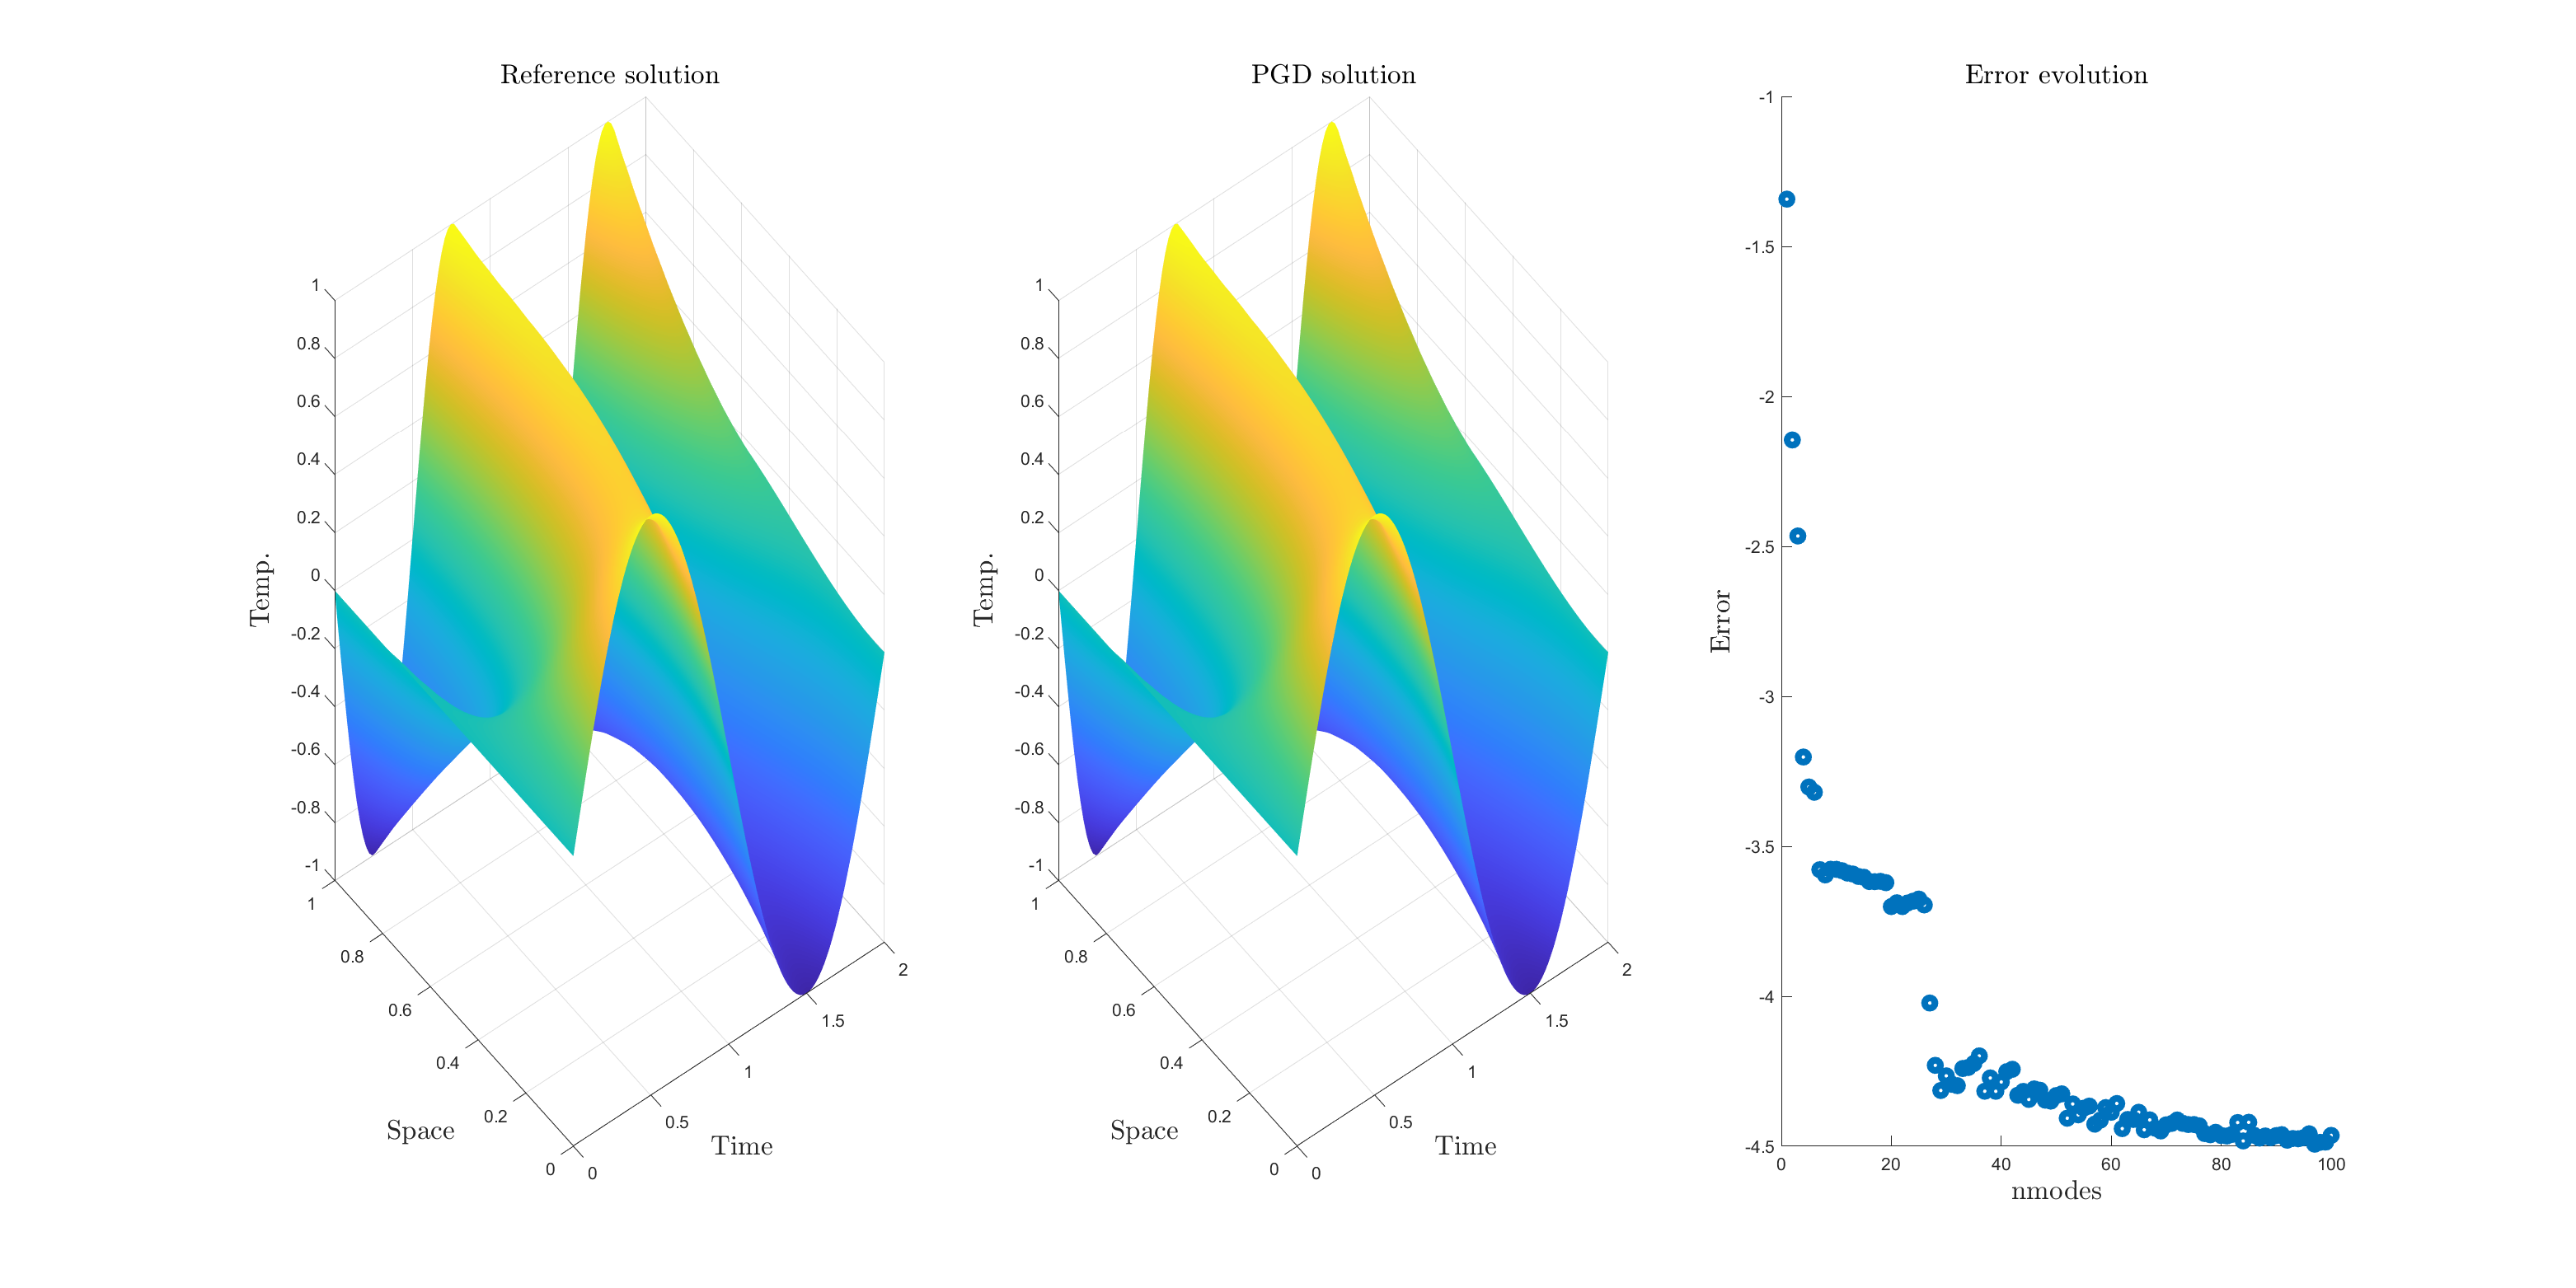
\includegraphics[width=\textwidth]{PGD_mode_100.png}
    \caption{Résultats PGD après 100 modes : solution de référence $U_{\text{ex}}$ (gauche),
    solution PGD $U_{\text{PGD}}$ (centre), évolution de $\log_{10}(\varepsilon)$
    en fonction du nombre de modes (droite).}
    \label{fig:pgd_mode100}
\end{figure}

\subsection{Validation du changement de variable}

La solution $U_1 = W + U_{CL}$ coïncide avec la référence à la précision machine
($\sim 10^{-12}$), ce qui valide l'approche par changement de variable.
Cette validation est essentielle avant de lancer l'algorithme PGD : elle garantit
que le problème modifié (\ref{eq:weq}) que nous résolvons est bien équivalent
au problème original (\ref{eq:heat}).

\subsection{Convergence PGD}

On observe sur la Figure~\ref{fig:pgd_mode100} que l'erreur décroît de manière
significative avec les premiers modes, puis se stabilise à un niveau bas.
Ce comportement reflète la faible dimension intrinsèque de la solution :
le problème de la chaleur avec des conditions aux limites régulières admet une
représentation efficace sur un faible nombre de modes séparés.
Cela est cohérent avec les attentes théoriques liées à la $n$-largeur de Kolmogorov :
si la $n$-largeur décroît vite, la PGD converge avec peu de modes.

% ============================================================
\section{Pour aller plus loin}
% ============================================================

\subsection{PGD avec phase de mise à jour}

\subsubsection{Motivation}

L'algorithme PGD glouton sans mise à jour présente une limitation fondamentale :
une fois qu'un mode est calculé, il reste figé pour toujours.
Cela peut mener à une convergence sous-optimale, car chaque mode est calculé
en supposant que les modes suivants corrigeront exactement les erreurs restantes.
Pour améliorer la convergence, on peut ajouter, après le calcul de chaque nouveau mode,
une phase de mise à jour qui recalcule tous les modes temporels simultanément.

\subsubsection{Phase d'orthonormalisation de Gram-Schmidt}

Après le calcul du $n$-ième mode $(\Lambda_n, \lambda_n)$, on orthonormalise
$\Lambda_n$ par rapport aux modes précédents via le procédé de Gram-Schmidt
dans le produit scalaire induit par $I_x$ :
\begin{equation}
    \Lambda_n \leftarrow \Lambda_n
    - \sum_{j=1}^{n-1} (\Lambda_n^\top I_x \Lambda_j)\, \Lambda_j
\end{equation}
En compensant les modes temporels pour maintenir l'égalité $W = \Lambda\lambda$ :
\begin{equation}
    \lambda_j \leftarrow \lambda_j
    + (\Lambda_n^\top I_x \Lambda_j)\, \lambda_n \quad \forall j < n
\end{equation}
Puis on renormalise : $\lambda_n \leftarrow \lambda_n \cdot \|\Lambda_n\|_{I_x}$ et
$\Lambda_n \leftarrow \Lambda_n / \|\Lambda_n\|_{I_x}$.
Cela garantit que la base spatiale $\{\Lambda_1, \ldots, \Lambda_n\}$ est
orthonormale pour $I_x$, ce qui simplifie et stabilise la phase de mise à jour.

\subsubsection{Phase de mise à jour par projection de Galerkin}

On cherche à mettre à jour simultanément tous les modes temporels
$\{\lambda_1(t), \ldots, \lambda_n(t)\}$ en projetant l'équation modifiée
(\ref{eq:weq}) sur la base spatiale courante.
En injectant $W = \sum_{r=1}^n \Lambda_r \lambda_r(t)$ et en testant par
$\Lambda_p$ pour $p = 1, \ldots, n$, on obtient le système couplé :
\begin{equation}
    \sum_{r=1}^n \left[(\Lambda_p^\top M \Lambda_r)\,\dot{\lambda}_r
    + (\Lambda_p^\top K \Lambda_r)\,\lambda_r\right]
    = \Lambda_p^\top Q_0(t) \quad \forall p = 1, \ldots, n
\end{equation}
Après discrétisation par Euler implicite, on résout à chaque pas de temps
un petit système de taille $n \times n$ :
\begin{equation}
    A\,\boldsymbol{\lambda}_{\text{up}}(:,i)
    = \boldsymbol{\Lambda}^\top Q_0(:,i)
    + M_{\text{mat}}\,\boldsymbol{\lambda}_{\text{up}}(:,i-1)
    \label{eq:update}
\end{equation}
où les matrices $A$ et $M_{\text{mat}}$ sont de taille $n \times n$,
calculées une seule fois par mode :
\begin{equation}
    A_{pr} = \frac{1}{\Delta t}\,\Lambda_p^\top M \Lambda_r
    + \Lambda_p^\top K \Lambda_r,
    \qquad
    M_{\text{mat},pr} = \frac{1}{\Delta t}\,\Lambda_p^\top M \Lambda_r
\end{equation}

\begin{lstlisting}
% Construction des matrices n x n (independantes du temps)
A_mat = zeros(mode, mode);
M_mat = zeros(mode, mode);
for p = 1:mode
    for r = 1:mode
        A_mat(p,r) = (1/dt)*LAMBDA(:,p)'*M*LAMBDA(:,r) ...
                     + LAMBDA(:,p)'*K*LAMBDA(:,r);
        M_mat(p,r) = (1/dt)*LAMBDA(:,p)'*M*LAMBDA(:,r);
    end
end
% Resolution du systeme en temps
lambdaup = zeros(mode, n_T);
for i = 2:n_T
    rhs = LAMBDA'*Q0(:,i) + M_mat*lambdaup(:,i-1);
    lambdaup(:,i) = A_mat \ rhs;
end
\end{lstlisting}

Grâce à cette mise à jour, la solution PGD devient une approximation de Galerkin
sur la base spatiale courante, ce qui améliore sensiblement la convergence par rapport
à la version sans mise à jour.

\subsubsection{Résultats}

La Figure~\ref{fig:pgd_update} montre les résultats de la PGD avec mise à jour
après 100 modes.

\begin{figure}[H]
    \centering
    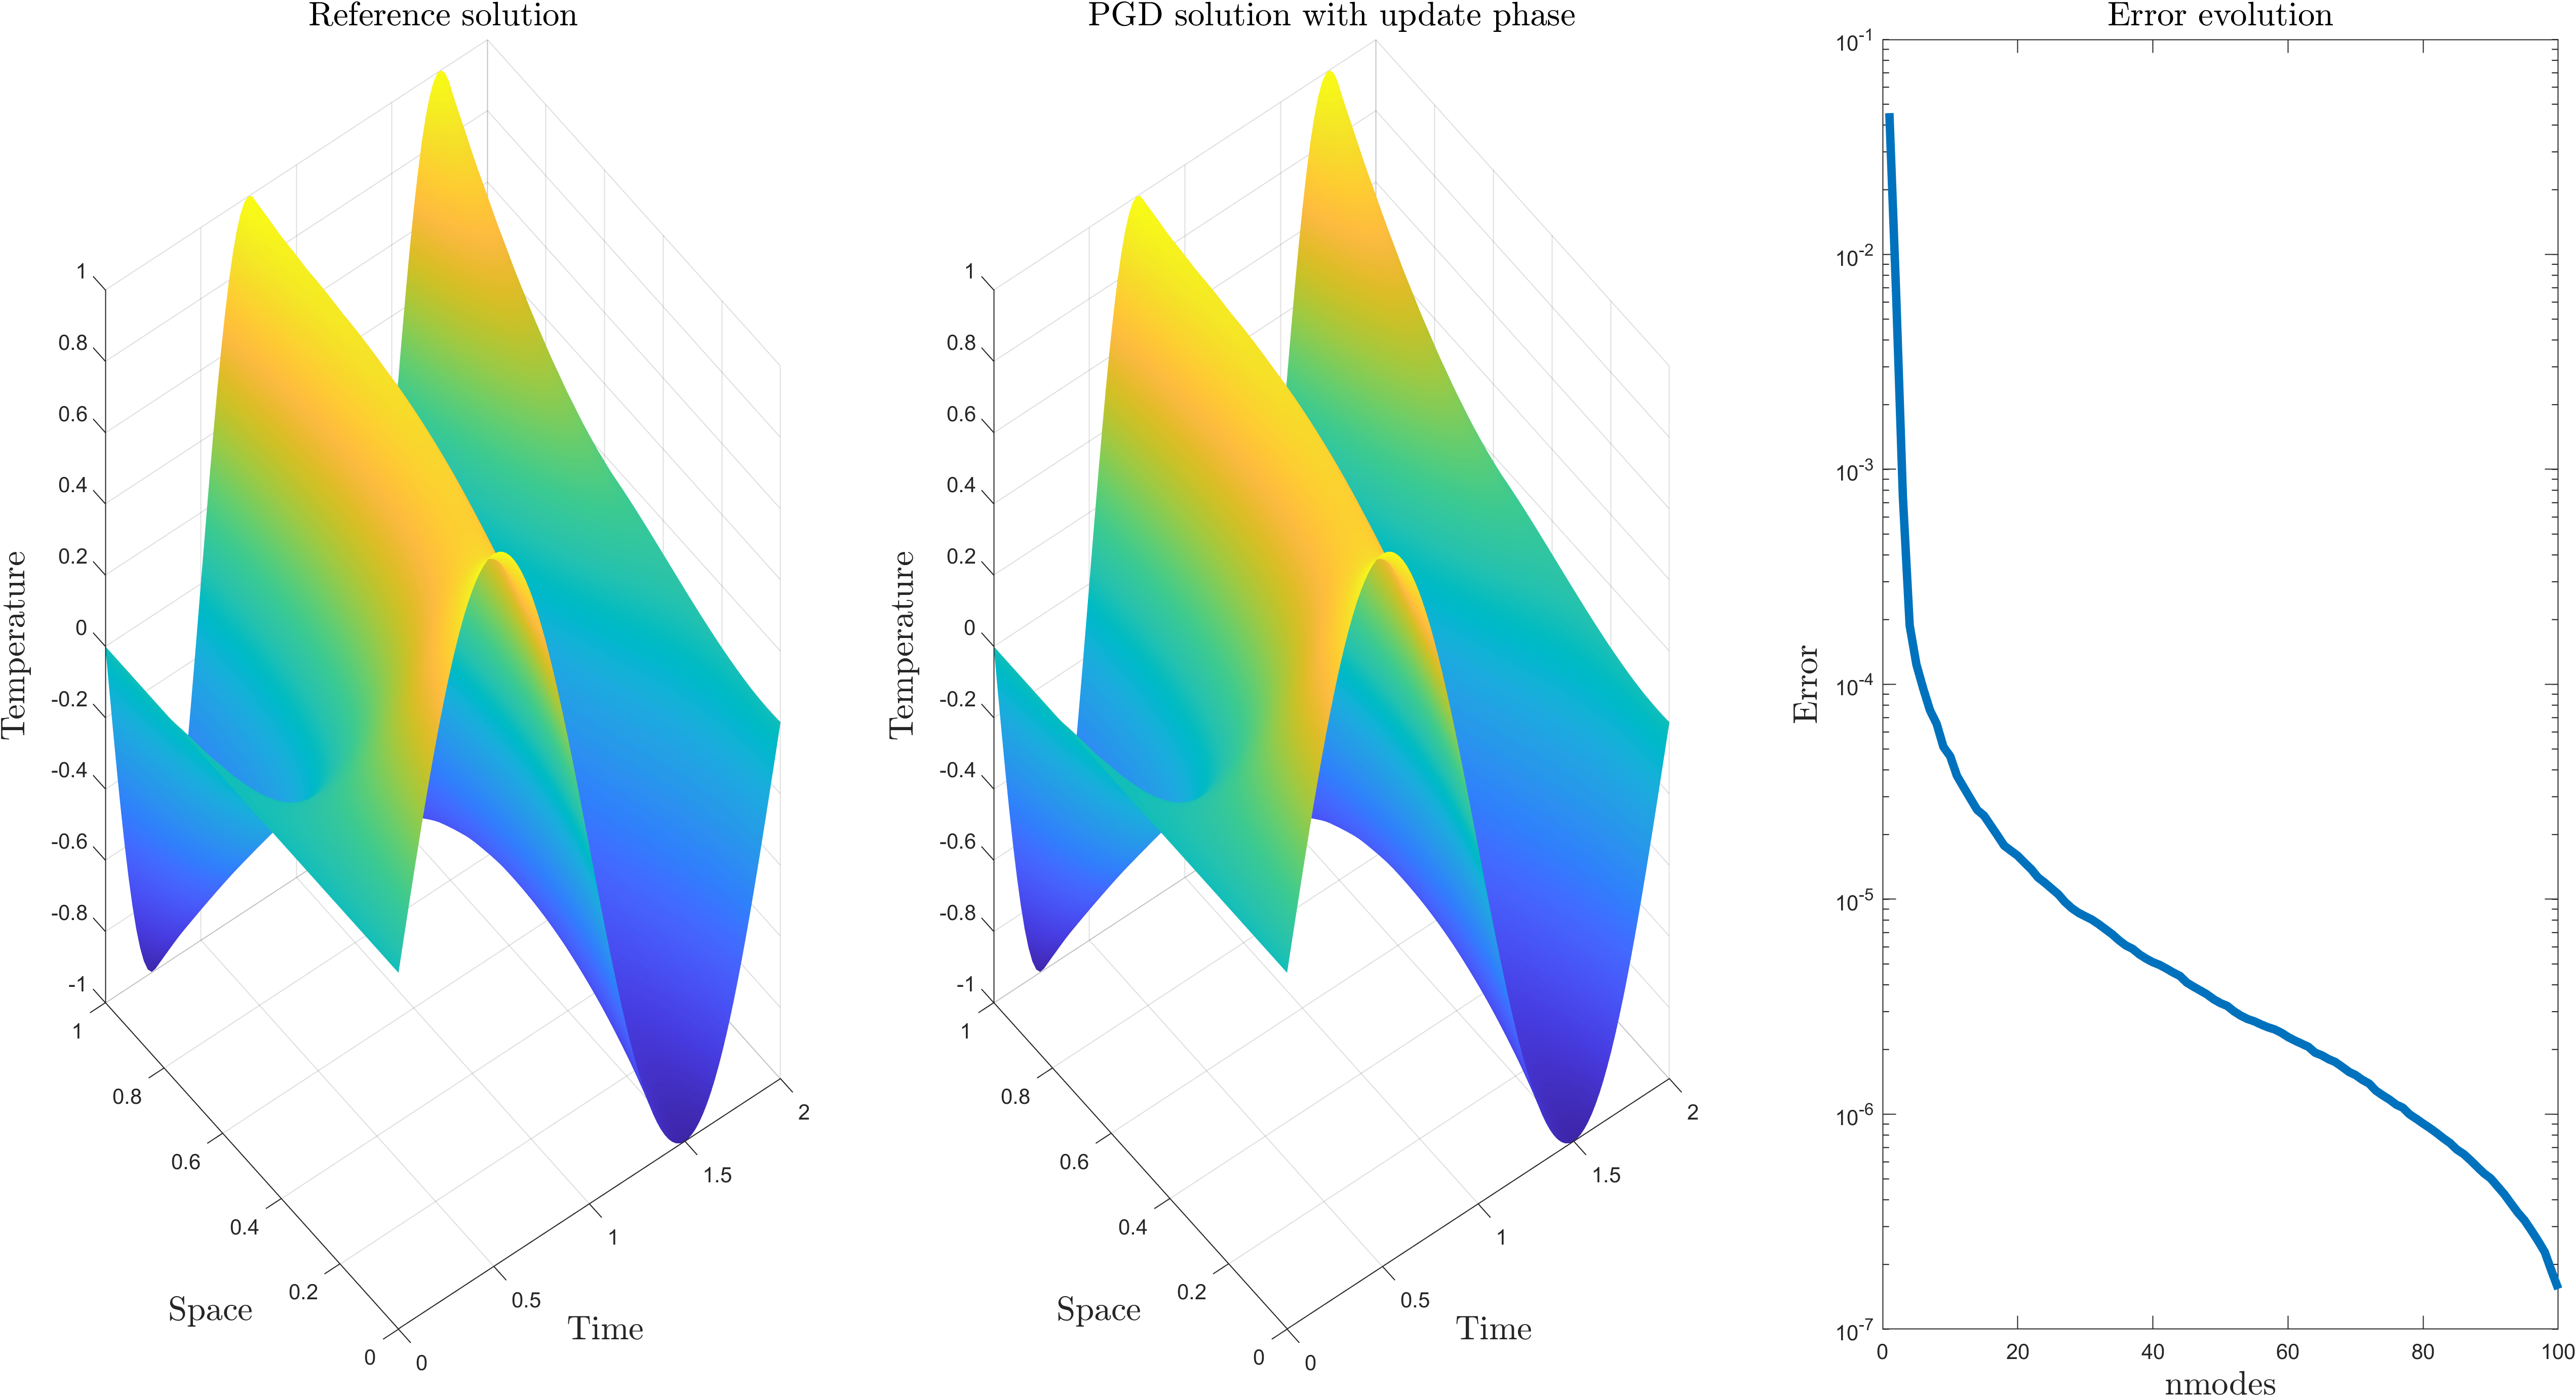
\includegraphics[width=\textwidth]{PGD_update_mode_100.png}
    \caption{PGD avec mise à jour après 100 modes : solution de référence (gauche),
    solution PGD avec mise à jour (centre), évolution de l'erreur (droite).}
    \label{fig:pgd_update}
\end{figure}

La Figure~\ref{fig:pgd_comparison} compare directement la convergence des deux variantes.
On constate que la phase de mise à jour accélère la convergence :
la PGD avec mise à jour atteint des niveaux d'erreur nettement inférieurs
avec le même nombre de modes.

\begin{figure}[H]
    \centering
    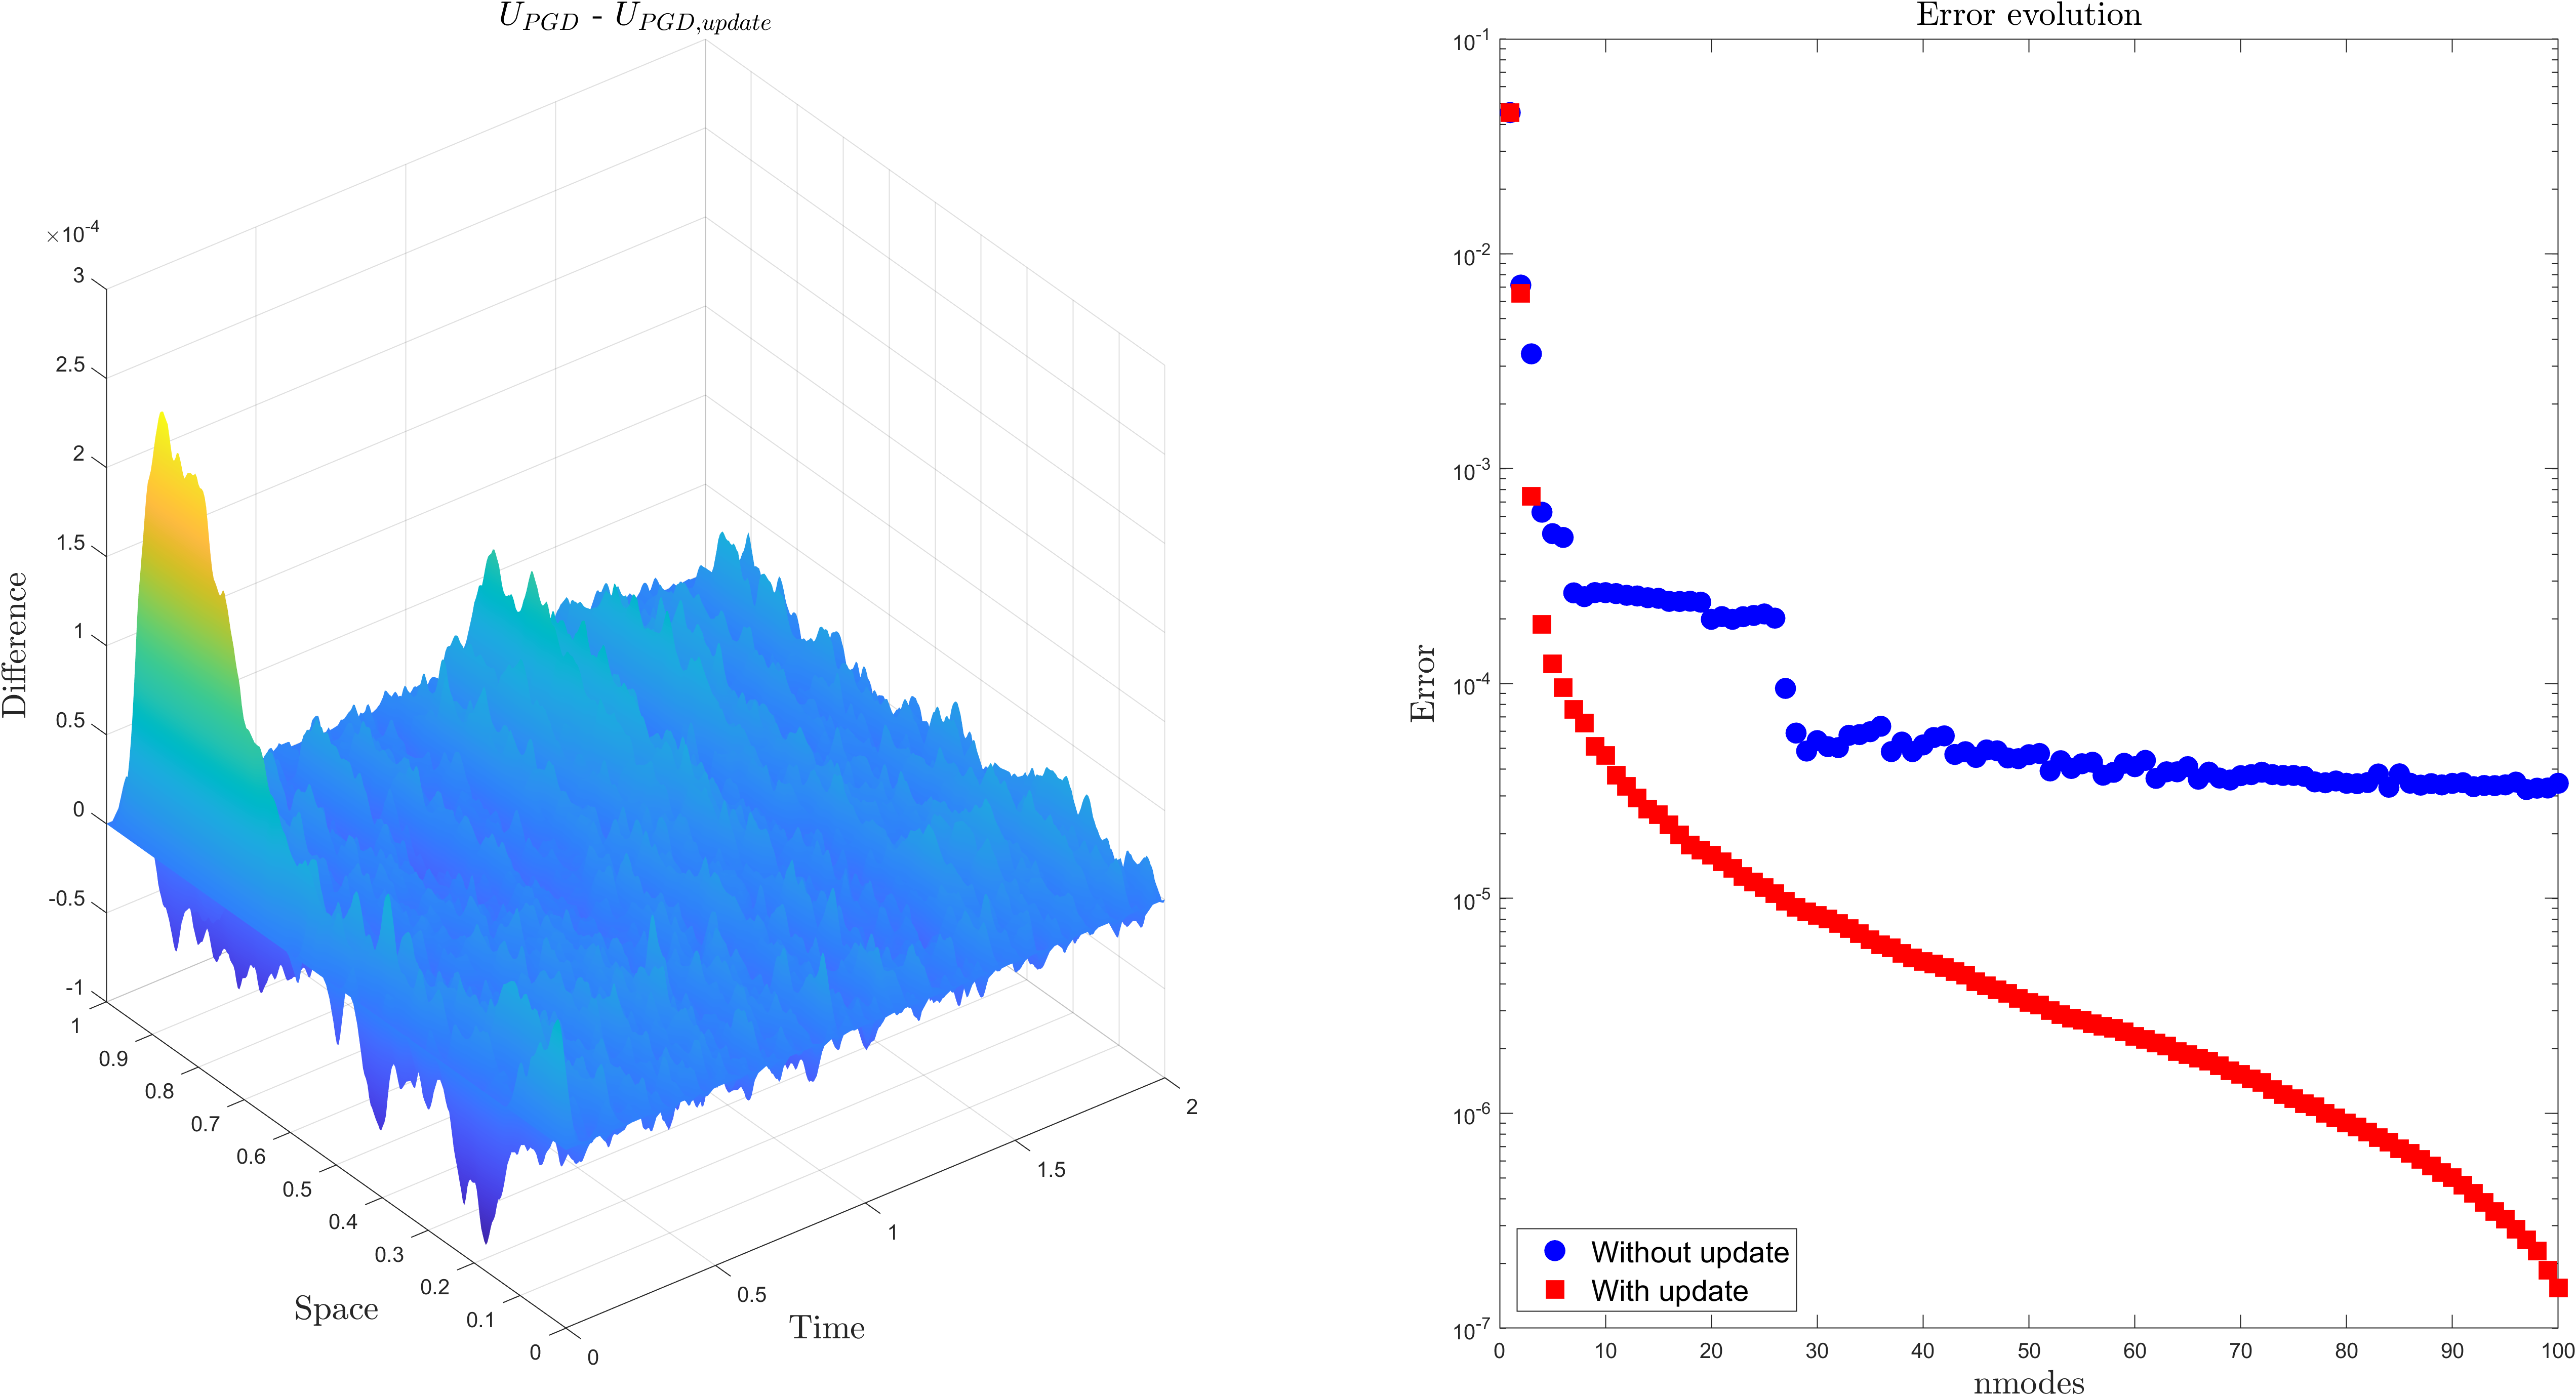
\includegraphics[width=\textwidth]{PGD_comparison.png}
    \caption{Comparaison PGD sans et avec mise à jour.
    Gauche : différence des champs $U_{\text{PGD}} - U_{\text{PGD,update}}$.
    Droite : courbes de convergence comparées -- sans mise à jour (bleu)
    vs.\ avec mise à jour (rouge).}
    \label{fig:pgd_comparison}
\end{figure}

\subsection{Comparaison avec la décomposition en valeurs singulières}

\subsubsection{La SVD comme borne optimale}

La décomposition en valeurs singulières (SVD) de la matrice
$U_{\text{ex}} \in \mathbb{R}^{N_x \times N_T}$ donne :
\begin{equation}
    U_{\text{ex}} = \sum_{i=1}^{\min(N_x,N_T)} \sigma_i\, u_i\, v_i^\top
    \label{eq:svd}
\end{equation}
où les $\sigma_i \geq 0$ sont les valeurs singulières rangées en ordre décroissant.
La troncature à $m$ termes :
\begin{equation}
    U_{\text{ex}}^{(m)} = \sum_{i=1}^{m} \sigma_i\, u_i\, v_i^\top
\end{equation}
est, d'après le théorème d'Eckart-Young, la meilleure approximation de rang $m$
de $U_{\text{ex}}$ au sens de la norme de Frobenius.
Elle constitue donc un minorant théorique de l'erreur pour toute méthode
de représentation séparée de rang $m$.

On notera que la SVD est une méthode a posteriori : elle nécessite de connaître
la solution complète $U_{\text{ex}}$ pour construire la décomposition.
En ce sens, elle n'est pas une méthode de réduction de modèle opérationnelle,
mais elle fournit une référence optimale pour évaluer les méthodes a priori comme la PGD.

\subsubsection{Résultats de la comparaison}

En MATLAB, le calcul SVD et l'erreur associée s'effectuent ainsi :
\begin{lstlisting}
[U_svd, S_svd, V_svd] = svd(Uex, 'econ');
for n = 1:n_modes
    Uex_svd = U_svd(:,1:n) * S_svd(1:n,1:n) * V_svd(:,1:n)';
    % ... calcul de l'erreur avec la meme norme L2 ...
end
\end{lstlisting}

La Figure~\ref{fig:pgd_svd} présente la comparaison des courbes de convergence
des trois méthodes, ainsi que les valeurs singulières de $U_{\text{ex}}$.

\begin{figure}[H]
    \centering
    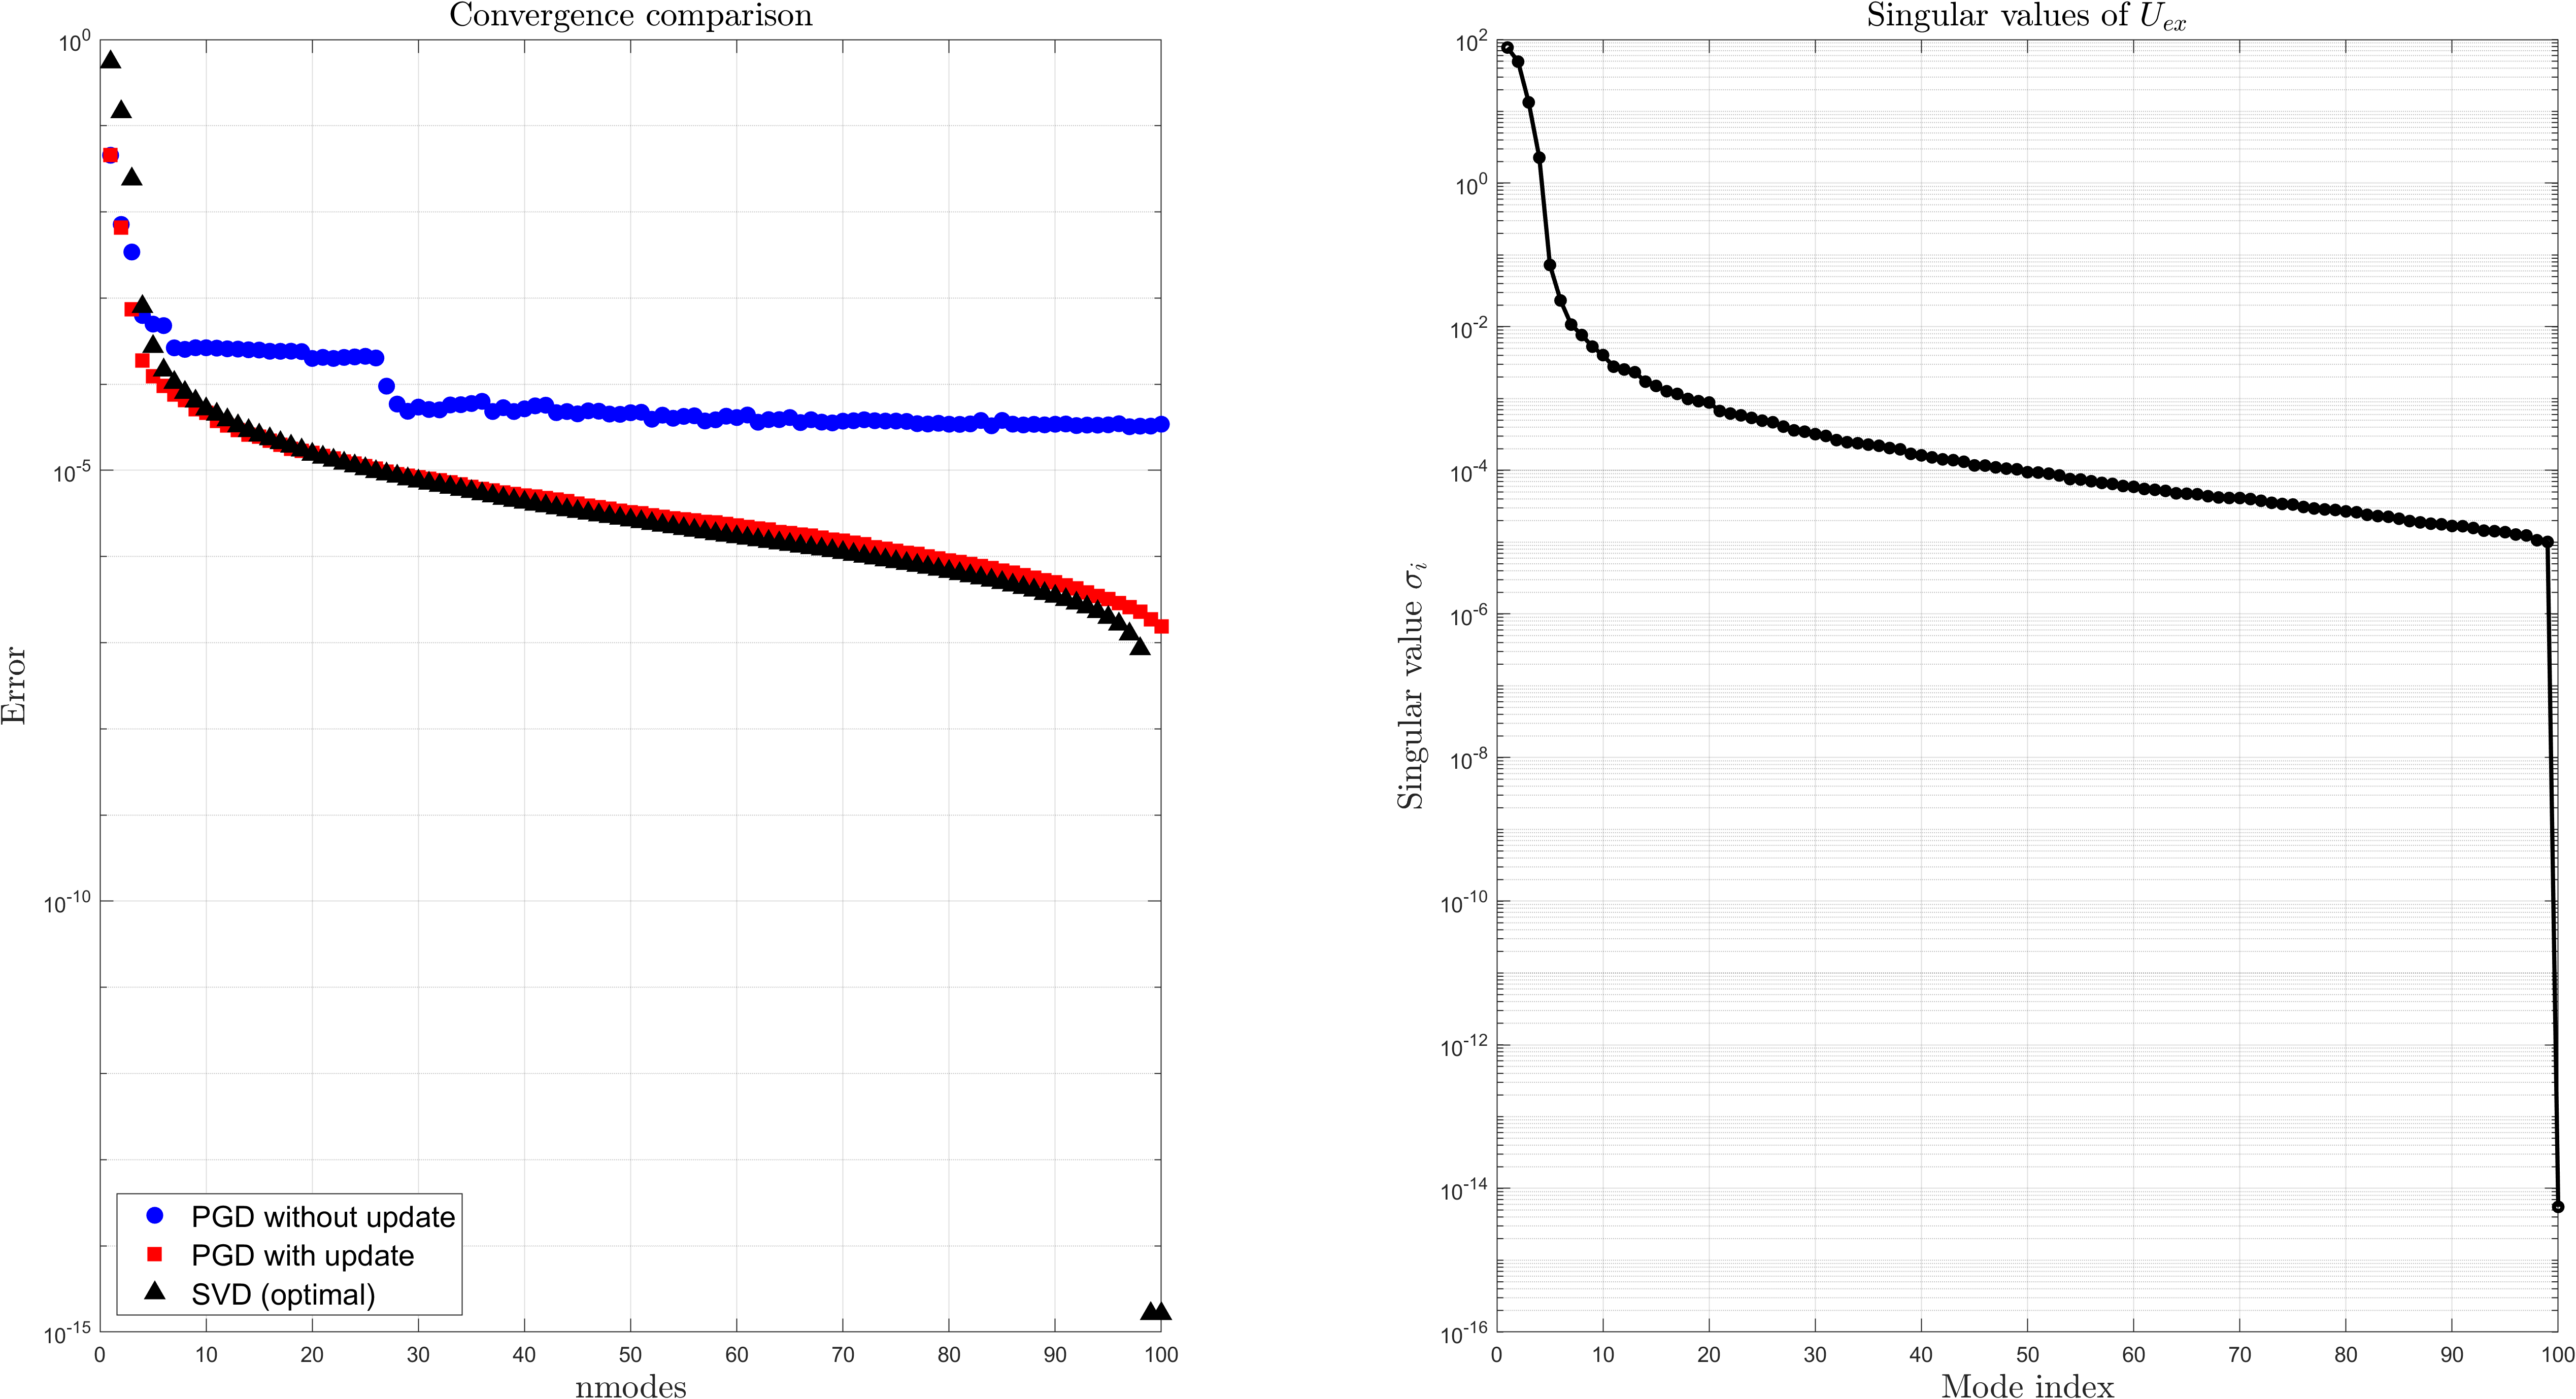
\includegraphics[width=\textwidth]{PGD_vs_SVD_comparison.png}
    \caption{Gauche : convergence comparée -- PGD sans mise à jour (bleu),
    PGD avec mise à jour (rouge), SVD optimale (noir).
    Droite : valeurs singulières $\sigma_i$ de $U_{\text{ex}}$.}
    \label{fig:pgd_svd}
\end{figure}

Plusieurs observations s'imposent.
La SVD converge plus vite que les deux variantes PGD avec le même nombre de modes :
c'est attendu puisqu'elle est optimale par construction.
La PGD avec mise à jour s'approche davantage de la borne SVD que la PGD sans mise à jour,
ce qui confirme l'intérêt de la phase de mise à jour.
Enfin, la décroissance rapide des valeurs singulières confirme la faible dimension
intrinsèque de la solution : l'essentiel de l'information est concentré dans
un faible nombre de modes séparés.
Ce résultat est directement lié à la notion de $n$-largeur de Kolmogorov :
une décroissance rapide des valeurs singulières implique que le sous-espace optimal
de dimension $n$ approxime très bien la variété des solutions.

\subsection{Analyse de complexité}

\subsubsection{Comparaison théorique}

Nous comparons ici le coût algorithmique des deux approches en termes
d'opérations flottantes.

\paragraph{Schéma EF + Euler implicite :}
À chaque pas de temps, nous résolvons un système linéaire de taille $N_x$.
Pour un système dense, le coût par résolution est $\mathcal{O}(N_x^2)$.
Sur $N_T$ pas de temps :
\begin{equation}
    \text{Coût}_{\text{EF+Euler}} = \mathcal{O}(N_T \cdot N_x^2)
\end{equation}

\paragraph{PGD (sans mise à jour) :}
Pour $m$ modes et $p$ itérations de point fixe en moyenne par mode :
\begin{itemize}
    \item $m \cdot p$ résolutions du problème EF spatial : coût $\mathcal{O}(N_x^2)$ chacune
    \item $m \cdot p$ résolutions de l'EDO temporelle : coût $\mathcal{O}(N_T)$ chacune
\end{itemize}
\begin{equation}
    \text{Coût}_{\text{PGD}} = \mathcal{O}\!\left(m \cdot p \cdot (N_x^2 + N_T)\right)
\end{equation}

La PGD est avantageuse lorsque $m \cdot p \ll N_T$, c'est-à-dire lorsque la solution
est bien représentée par un faible nombre de modes séparés.
Le rapport de coût s'écrit :
\begin{equation}
    \frac{\text{Coût}_{\text{PGD}}}{\text{Coût}_{\text{EF+Euler}}}
    \approx \frac{m \cdot p}{N_T}
    \quad (\text{pour } N_x^2 \gg N_T)
\end{equation}
Avec $m = 20$ modes, $p = 5$ itérations, et $N_T = 100$ pas de temps,
ce rapport vaut $20 \times 5 / 100 = 1$.
Pour $N_T = 1000$, il chute à $0.1$ : la PGD est dix fois moins chère.

\subsubsection{Vérification numérique}

Pour vérifier cette analyse, nous avons calculé numériquement le nombre d'opérations
théorique en faisant varier $N_x$ et $N_T$ séparément avec les paramètres :
$m = 20$ modes, $p = 5$ itérations de point fixe en moyenne.

\begin{lstlisting}
% Cout theorique FEM + Euler : O(n_T * n_X^2)
cost_fem = nt * nx^2;
% Cout theorique PGD : O(n_m * n_iter_fp * (n_X^2 + n_T))
cost_pgd = n_m * n_iter_fp * (nx^2 + nt);
\end{lstlisting}

La Figure~\ref{fig:complexity} montre les courbes de complexité en échelle log-log.

\begin{figure}[H]
    \centering
    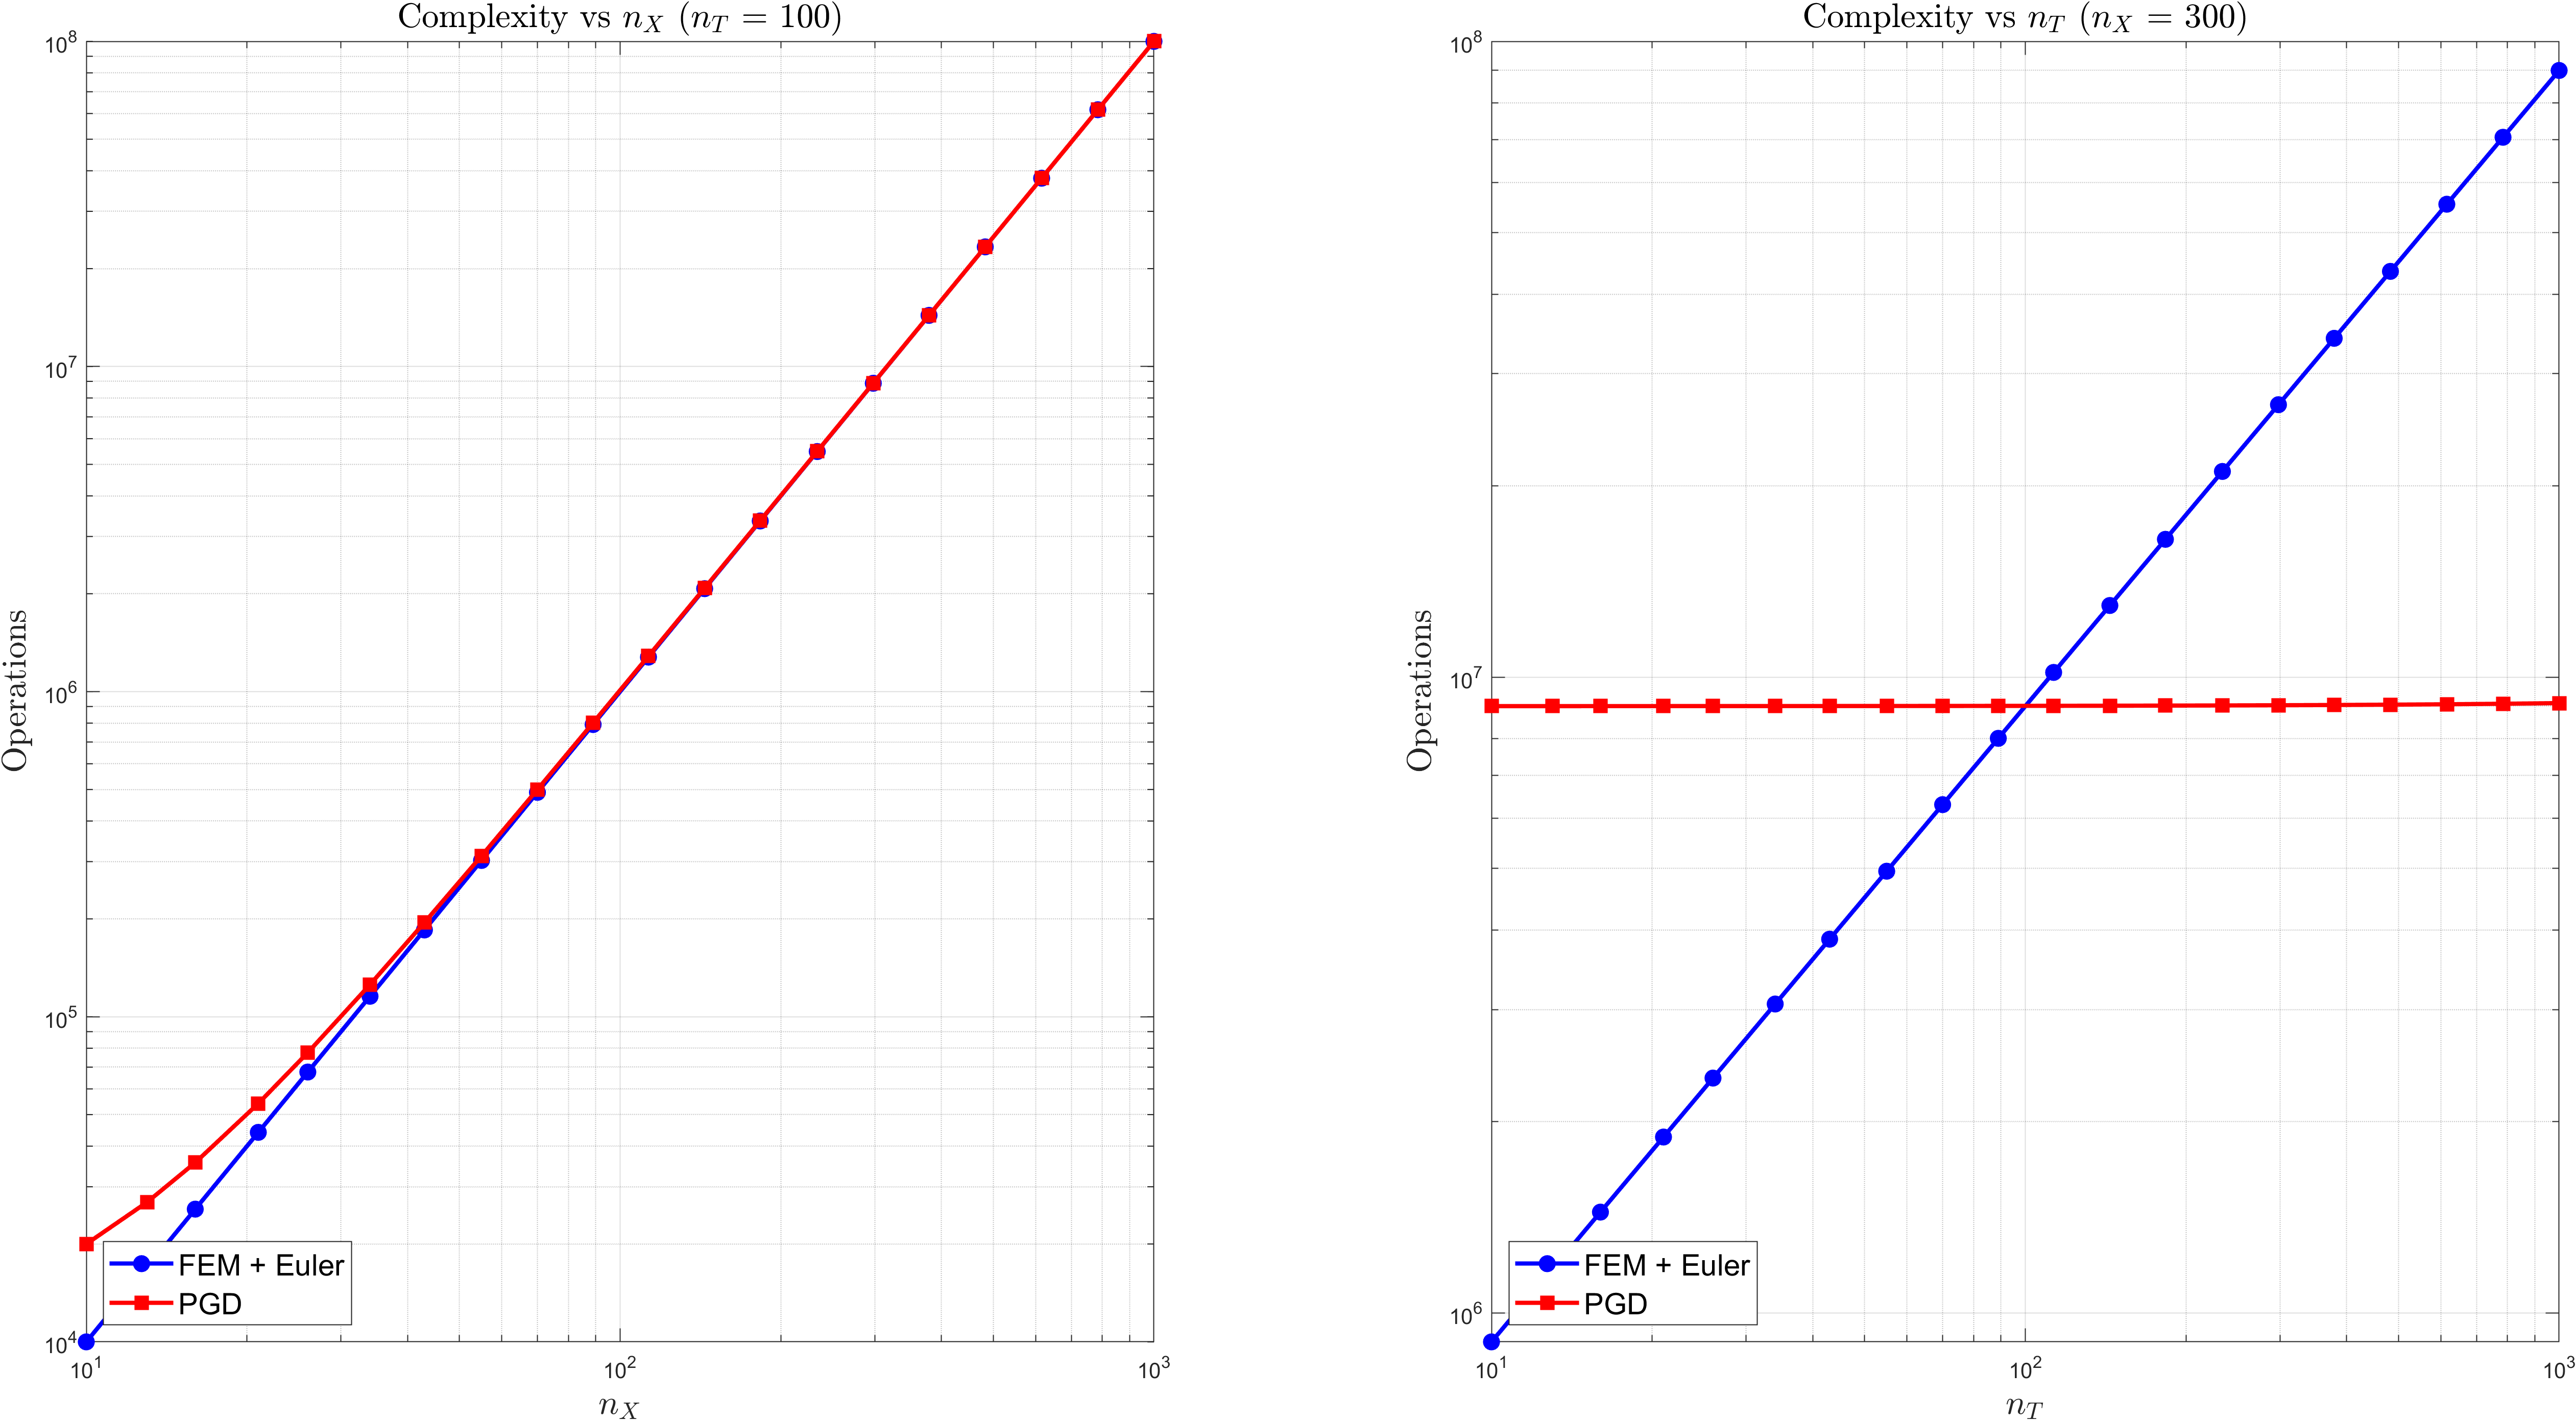
\includegraphics[width=\textwidth]{PGD_complexity_comparison.png}
    \caption{Comparaison des complexités algorithmiques : EF+Euler (bleu) vs.\ PGD (rouge).
    Gauche : en fonction de $N_x$ ($N_T = 100$ fixé).
    Droite : en fonction de $N_T$ ($N_x = 300$ fixé).}
    \label{fig:complexity}
\end{figure}

On observe clairement que :
\begin{itemize}
    \item En fonction de $N_x$, les deux méthodes affichent la même pente en échelle
    log-log ($\mathcal{O}(N_x^2)$), ce qui est attendu : les deux nécessitent
    des résolutions de systèmes linéaires spatiaux de taille $N_x$.
    Le décalage vertical entre les courbes correspond simplement au facteur multiplicatif
    $m \cdot p$ vs.\ $N_T$.

    \item En fonction de $N_T$, le coût EF+Euler croît linéairement (pente 1 en log-log),
    tandis que le coût PGD reste pratiquement constant (pour un nombre de modes fixé).
    C'est ici que la PGD prend tout son avantage : plus $N_T$ est grand,
    plus le gain relatif en faveur de la PGD est important.
\end{itemize}

Ces observations confirment que la PGD est particulièrement adaptée aux problèmes
avec un grand nombre de pas de temps et une solution de faible dimension intrinsèque,
ce qui est le cas typique pour notre équation de la chaleur.

% ============================================================
\section{Conclusion}
% ============================================================

Cette séance pratique nous a permis d'implémenter et de tester la méthode PGD
comme technique de réduction de modèle a priori pour la résolution de l'équation
de la chaleur 1D instationnaire. Les points essentiels que nous retenons sont
les suivants.

Le \textbf{changement de variable} $U = U_{CL} + W$ transforme le problème avec des
conditions aux limites non homogènes en un problème à conditions homogènes,
indispensable pour chercher $W$ sous forme séparée.

\textbf{L'alternance de point fixe} entre un problème EF spatial et une EDO temporelle
permet de calculer chaque mode de manière efficace, sans assembler ni résoudre
le système espace-temps global.

\textbf{L'algorithme glouton} construit les modes un par un, chacun corrigeant le résidu
laissé par les modes précédents. Sa convergence rapide confirme la faible dimension
intrinsèque de la solution pour ce type de problème.

La \textbf{phase de mise à jour} par projection de Galerkin améliore sensiblement la
convergence en recalculant simultanément tous les modes temporels sur la base spatiale
courante. Elle rapproche la PGD de la borne optimale fournie par la SVD.

La \textbf{comparaison avec la SVD} montre que la PGD avec mise à jour approche la
décomposition optimale, ce qui valide à la fois l'implémentation et l'intérêt de la
méthode. La décroissance rapide des valeurs singulières de $U_{\text{ex}}$ confirme
que le problème est intrinsèquement de faible dimension.

Enfin, l'\textbf{analyse de complexité} confirme l'avantage de la PGD pour les problèmes
avec un grand nombre de pas de temps : le coût de la PGD ne croît pas avec $N_T$
(pour un nombre de modes fixé), contrairement au schéma EF+Euler.
Cet avantage devient décisif dans des contextes multi-paramétriques ou temps-réel,
où la même base réduite peut être réutilisée pour de nombreuses configurations.

\end{document}
